\documentclass[11pt]{article}
\usepackage[margin=.78in]{geometry}
\usepackage{amsmath,amssymb,graphicx,booktabs,hyperref}
\setlength{\parindent}{0pt}\setlength{\parskip}{6pt}
\begin{document}
{\LARGE Actual twist transfer over $\mathbf F_{37}$}\\
2026-10-30\quad PR2381\quad fixed public synthetic fixture

Let $E:y^2=x^3+7x+19$ and $T:y^2=x^3+28x+33$, the actual monic
 twist with nonsquare $d=35$. Each has 38 rational points.
The fixed lexicographic rule selects $P=(1,8)$ and $U=(32,29)$,
both of order 19. These are unregistered model tuples; no endomorphism-ring
classification is inferred.
\[
\Phi(x,y)=\left(x+\frac{18}{x-4},\ y\left(1-\frac{18}{(x-4)^2}\right)\right),
\]
\[
D(x,y)=\left(28\left(x+\frac{35}{x-29}\right),\ 14y\left(1-\frac{35}{(x-29)^2}\right)\right).
\]
Origins and the respective kernel points $(4,0)$ and $(29,0)$ map to the origin.
The inverse on the order-19 subgroups is $I=[10]D$.
\begin{center}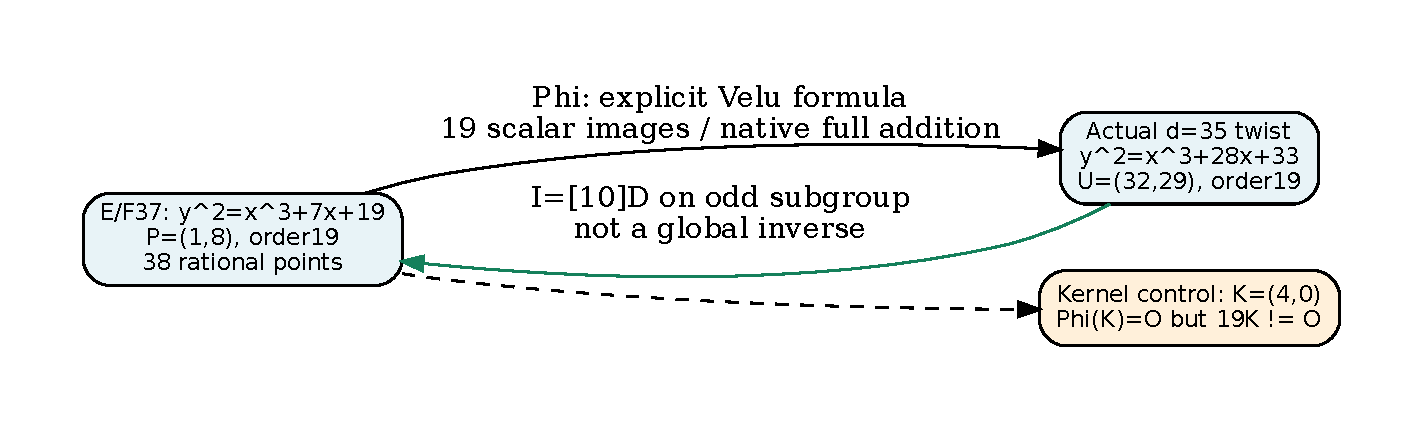
\includegraphics[width=\linewidth,height=2.15in,keepaspectratio]{bridge.pdf}\end{center}
\textbf{Independent native verification.} All $38+38$ point images, both
compositions $=[2]$, 2888 addition pairs, and 19 scalar images/inverses pass.
The false inverse $[9]D$ differs on all 18 nonzero subgroup points.

\textbf{Lean result.} The unmodified scoped gate passes 19 public named
theorems and 22 audited declarations, with zero failing or extra trusted/native
axioms. The actual Mathlib nonsingular points use the displayed coordinate
formulas. Lean checks equations, order, scalar transport, subgroup addition,
inverse identities, and a necessary coefficient obstruction to a short-model
change. For an actual unknown source point $Q$ and $n\in\mathrm{Fin}\,19$:
\[
 (\exists i\in\mathrm{Fin}\,19,\ Q=iP)\ \Longrightarrow\
 [\Phi(Q)=nU\ \Longleftrightarrow\ Q=nP].
\]
This does not give a solver the unknown index. Global inversion is false at
the source 2-torsion point. Generic geometric classification is not formalized.

\clearpage
{\Large Full size-two policy frontier}
\begin{center}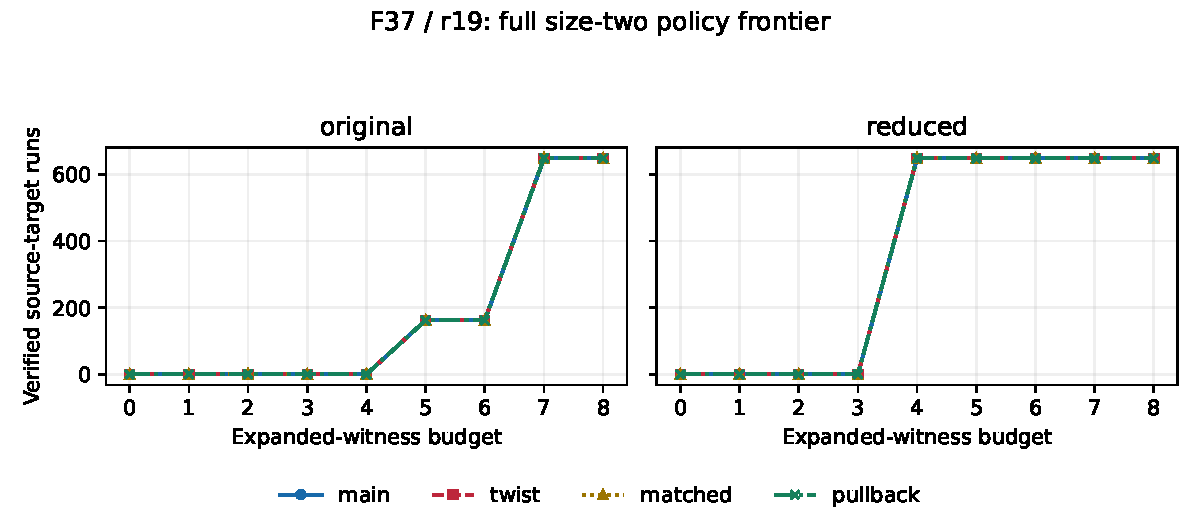
\includegraphics[width=\linewidth]{frontier.pdf}\end{center}
\textbf{Figure.} Native-emitted counts for 36 policies and 18 source points per
role and cap. Curves may overlap. These are exact finite values; no timing or
sampling uncertainty is inferred.

All 144 arms, including matched and pullback controls, run both encodings at
caps 0--8: 2592 configurations and 46656 separate target attempts. The latter
repeat 18 source points across policies, encodings and budgets.

\begin{center}\begin{tabular}{lr}\toprule
Independently reconstructed outcome & Count\\\midrule
Verified original-source recoveries &19440\\
Blocked public-log setups &1512\\
Policy/target/budget pair records &3779136\\
Higher rank, lower requested cap, recovery admitted &55230\\
Such records beating the strongest source policy &0\\
Changed controls rejected, no receipt &10\\
Shared backend tests passed &22\\\bottomrule\end{tabular}\end{center}

The 55230 records are pair comparisons, not distinct target wins. A lower
requested cap need not mean a lower actual solving degree. None of these gains
survives comparison with the strongest canonical source policy at the comparison
budget. Stationary yield, intrinsic regularity, runtime and complete-cost gains
remain unestablished. The smaller F13 cohort is not a matched speed reference.

\clearpage
{\Large Execution, evidence and next test}

\textbf{Algebraic instrument.} New F37/r19 sources receive three inputs:
$S_3$ and both product-membership constraints. Flat Macaulay rows carry exact
original-input witnesses. A unit or bounded Buchberger certificate must pass
before root extraction. Both matrix degree and expanded verification-witness
degree fit the rung. Above-bound shifts are denied before construction; an
unknown cap result admits no roots or rows. A smaller already-computed witness
is retained only for the identical polynomial within one solve.

Public setup derives logs only from admitted relations and checks the actual
base points. Incomplete rank blocks every target. Recovery receives actual
unknown $Q$, makes fresh shifted solves, retains every failed or identity shift
and sign lift, and verifies the scalar on the original $E/P$. Output-reference
binding follows each fresh solve and is unpriced. Direct enumeration is a
separate generic decomposition reference, with no named matrix degree.
Setup, allocation, field/group operations and verification lack a complete price.

\textbf{Preservation and failures.} Complete producer and independent auditor
paths pass. Nine census corruptions and one false-inverse payload genuinely
change and reject with exit 101 and no receipt. All canonical cases, altered
payloads, control reconstruction, raw commands/logs and proof receipts remain.
The 18 prior polynomial identity records are unchanged; no new identity or
combined/global proof audit is claimed.

The first Lean setup failed before elaboration while cloning Mathlib. An exact
pinned dependency cache was then reused without changing the gate. Attempt 02
has an explicit successful gate exit and PASS audit despite an outer PTY exit
discrepancy. An unchanged-source repeat explicitly returned zero/PASS; both
records remain. A copied F13-ordering phrase in the frozen protocol has a dated
metadata erratum. The new F37 scope was already explicit in the question, arms,
parameters, Markdown, sources and coverage assertions. No criterion changed.

\textbf{Next test.} Use all size-three bases over this verified route: 84
canonical policies per curve plus matched and pullback controls. A new protocol
and instrument are required. Since $S_3$ has degree at most two per variable,
cubic membership reduction leaves it unchanged; this must be an explicit
encoding-equality control. This next experiment is not implemented or run here.

The PR stays open, non-draft, with auto-merge off. Registry, incomplete library
suite, naming, required CI, review, integration and Conductor holds remain.
The scientific window was 13:40--14:40 UTC, with two local workers and 600-second
command caps. No paid resource or arbitrary result upload was used.

\small Primary source: Sage isogeny blob 972f4116\ldots, Kohel/V\'elu formulas
and sum helper. Full source links, proof map, hashes and replay instructions are
in the adjacent README and validation directory.
\end{document}
